\documentclass[aspectratio=169,xcolor=dvipsnames]{beamer}

%==============================================================================
% PACKAGES & THEME
%==============================================================================
\usepackage[utf8]{inputenc}
\usepackage[T1]{fontenc}
\usepackage{amsmath,amssymb,mathtools}
\usepackage{graphicx}
\usepackage{booktabs}
\usepackage{hyperref}
\usepackage{xcolor}
\usepackage{tikz}
\usepackage{subcaption}
\usepackage[authoryear]{natbib}
\usepackage{multirow}

\usetikzlibrary{shapes.geometric, arrows, positioning, shadows, fit}

% Modern color palette
\definecolor{MainBlue}{HTML}{1A237E}
\definecolor{AccentTeal}{HTML}{009688}
\definecolor{AccentOrange}{HTML}{FF6D00}
\definecolor{SoftGrey}{HTML}{F5F5F5}
\definecolor{DarkGrey}{HTML}{424242}

\usetheme{metropolis} % Clean, modern theme
\metroset{block=fill, sectionpage=progressbar, progressbar=frametitle}

\setbeamercolor{palette primary}{bg=MainBlue, fg=white}
\setbeamercolor{progress bar}{fg=AccentTeal}
\setbeamercolor{frametitle}{bg=MainBlue, fg=white}

% Custom commands
\newcommand{\I}[1]{\mathbf{1}\{#1\}}
\newcommand{\E}{\mathbb{E}}

%==============================================================================
% TITLE DATA
%==============================================================================
\title{Forecasting Under Structural breaks}
\subtitle{A Concise Monte Carlo Synthesis}
\author{Aadya Khatavkar \and Bakhodir Izzatulloev \and Mahir Beylerov}
\date{Winter Semester 2025/26}
\institute{University of Bonn}

\begin{document}

% 1. Title Page
\begin{frame}[plain]
  \titlepage
\end{frame}

% 2. Motivation: The "Infographic" Slide
\begin{frame}{Motivation: Why Adapt?}
  \begin{columns}
    \begin{column}{0.6\textwidth}
      \begin{itemize}
        \item \textbf{The Reality:} Economic data is rarely stable (Crisis, Policy, Tech).
        \item \textbf{The Failure:} Global models average across regimes $\to$ Massive Bias.
        \item \textbf{The Goal:} Navigate shifts in \textbf{Mean}, \textbf{Variance}, and \textbf{Persistence}.
      \end{itemize}
    \end{column}
    \begin{column}{0.4\textwidth}
      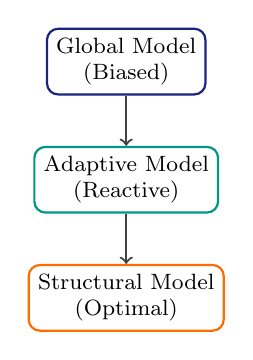
\begin{tikzpicture}[node distance=1.5cm, every node/.style={fill=white, font=\footnotesize}, align=center]
        \node (a) [draw=MainBlue, thick, rounded corners] {Global Model\\(Biased)};
        \node (b) [below of=a, draw=AccentTeal, thick, rounded corners] {Adaptive Model\\(Reactive)};
        \node (c) [below of=b, draw=AccentOrange, thick, rounded corners] {Structural Model\\(Optimal)};
        \draw [->, thick, DarkGrey] (a) -- (b);
        \draw [->, thick, DarkGrey] (b) -- (c);
      \end{tikzpicture}
    \end{column}
  \end{columns}
  \vspace{0.5cm}
  \begin{block}{Research Question}
    Which strategy minimizes RMSE when the "rules" of the system change?
  \end{block}
\end{frame}

% 3. Literature Pillars (Concise table)
\begin{frame}{Literature Review: Key Authors}
  \begin{center}
    \renewcommand{\arraystretch}{1.2}
    \begin{tabular}{lp{10cm}}
      \toprule
      \textbf{Pillar} & \textbf{Foundational Contribution} \\
      \midrule
      \textcolor{MainBlue}{\textbf{Evidence}} & \textbf{Stock \& Watson (1996)}: Instability is pervasive in macro data. \\
      \textcolor{MainBlue}{\textbf{Detection}} & \textbf{Bai \& Perron (1998, 2003)}: Identifying multiple unknown breaks. \\
      \textcolor{MainBlue}{\textbf{Adaptation}} & \textbf{Rossi (2013); Pesaran (2013)}: Frameworks for rolling windows. \\
      \textcolor{MainBlue}{\textbf{Regimes}} & \textbf{Hamilton (1989)}: Markov-Switching for recurring shifts. \\
      \textcolor{MainBlue}{\textbf{Special}} & \textbf{Wang et al. (2013)}: Distinguishing breaks from long memory. \\
      \bottomrule
    \end{tabular}
  \end{center}
\end{frame}

% 4. The Unified DGP Framework
\begin{frame}{The Simulation Design: Three Break Archetypes}
  \[ y_t = c_t + \phi_t y_{t-1} + \varepsilon_t, \quad \varepsilon_t \sim \text{Dist}(0, \sigma_t^2) \]
  
  \begin{columns}
    \begin{column}{0.33\textwidth}
      \begin{block}{1. Mean Shift}
        \centering
        $c_0 \xrightarrow{T_b} c_1$ \\
        \textit{Level Shifts}
      \end{block}
    \end{column}
    \begin{column}{0.33\textwidth}
      \begin{block}{2. Variance Shift}
        \centering
        $\sigma_1 \xrightarrow{T_b} \sigma_2$ \\
        \textit{Volatility Shocks}
      \end{block}
    \end{column}
    \begin{column}{0.33\textwidth}
      \begin{block}{3. Parameter Shift}
        \centering
        $\phi_1 \xrightarrow{T_b} \phi_2$ \\
        \textit{Persistence Breaks}
      \end{block}
    \end{column}
  \end{columns}
  \vspace{0.3cm}
  \begin{itemize}
    \item \textbf{Setup:} $T=300$, $1000$ iterations, Gaussian vs. Heavy-tailed ($t$-dist).
    \item \textbf{Extensions:} Seasonality (SARIMA) and Recurring breaks (Markov).
  \end{itemize}
\end{frame}

% 5. Methodology Comparison
\begin{frame}{Strategy Portfolio: 15+ Methods}
  \begin{center}
    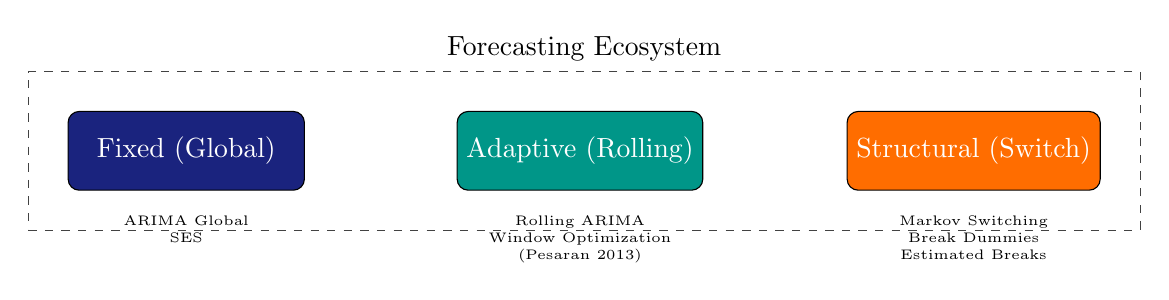
\begin{tikzpicture}
      \node[draw, fill=MainBlue, text=white, rounded corners, minimum height=1cm, minimum width=3cm] (fixed) at (0,0) {Fixed (Global)};
      \node[draw, fill=AccentTeal, text=white, rounded corners, minimum height=1cm, minimum width=3cm] (adapt) at (5,0) {Adaptive (Rolling)};
      \node[draw, fill=AccentOrange, text=white, rounded corners, minimum height=1cm, minimum width=3cm] (struc) at (10,0) {Structural (Switch)};
      
      \node[below=0.2cm of fixed, font=\tiny, align=center] {ARIMA Global\\SES};
      \node[below=0.2cm of adapt, font=\tiny, align=center] {Rolling ARIMA\\Window Optimization\\(Pesaran 2013)};
      \node[below=0.2cm of struc, font=\tiny, align=center] {Markov Switching\\Break Dummies\\Estimated Breaks};
      
      \node[draw=DarkGrey, dashed, fit={(fixed) (adapt) (struc)}, inner sep=0.5cm, label=above:Forecasting Ecosystem] {};
    \end{tikzpicture}
  \end{center}
\end{frame}

% 6. Result: Variance Breaks
\begin{frame}{Result 1: Volatility Shifts}
  \begin{columns}
    \begin{column}{0.5\textwidth}
      \begin{itemize}
        \item \textbf{Winner:} \textbf{GARCH(1,1)} adapts fastest to variance shifts.
        \item \textbf{Insight:} Rolling windows must be small ($w < 50$) to capture sudden volatility jumps.
        \item \textbf{Loss Surface:} Clear U-shape showing window size trade-off.
      \end{itemize}
    \end{column}
    \begin{column}{0.5\textwidth}
       \includegraphics[width=\textwidth]{../../figures/variance/variance_forecasts_comparison.png}
    \end{column}
  \end{columns}
\end{frame}

% 7. Result: Mean Breaks & Seasonality (Bakhodir)
\begin{frame}{Result 2: Level Shifts \& Seasonality}
  \begin{columns}
    \begin{column}{0.5\textwidth}
       \includegraphics[width=\textwidth]{../../figures/mean/single_break_RMSE.png}
    \end{column}
    \begin{column}{0.5\textwidth}
      \begin{itemize}
        \item \textbf{Bakhodir's Extension:} SARIMA methods explicitly modeling seasonality + breaks.
        \item \textbf{Finding:} \textbf{SARIMA Rolling} beats global by 15-20\% RMSE.
        \item \textbf{Oracle:} Known break dates reduce RMSE by an additional 10\%.
      \end{itemize}
    \end{column}
  \end{columns}
\end{frame}

% 8. Result: Persistence & Markov Switching
\begin{frame}{Result 3: Persistence Shifts}
  \begin{columns}
    \begin{column}{0.4\textwidth}
      \begin{itemize}
        \item \textbf{Hardest Case:} Shift in $\phi$ (memory).
        \item \textbf{Markov Switching:} Shines in recurring breaks with high persistence ($p \ge 0.97$).
        \item \textbf{Grid Search:} Estimating break dates is viable but noisier than rolling windows.
      \end{itemize}
    \end{column}
    \begin{column}{0.6\textwidth}
       \includegraphics[width=\textwidth]{../../figures/parameter/parameter_persistence_analysis.png}
    \end{column}
  \end{columns}
\end{frame}

% 9. Optimization: Pesaran (2013) Window Search
\begin{frame}{Optimizing Adaptivity}
  \textbf{Goal:} Choose window size $w^*$ without knowing break date.
  
  \begin{center}
    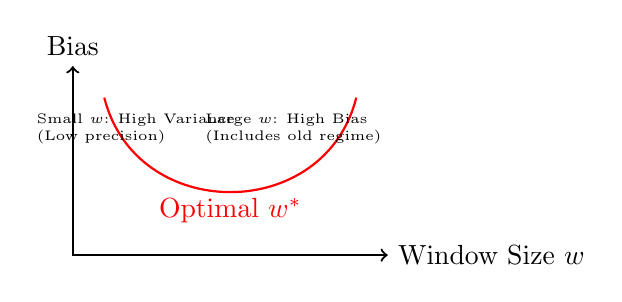
\begin{tikzpicture}[scale=0.8]
      \draw[thick, <->] (0,3) node[above]{Bias} -- (0,0) -- (5,0) node[right]{Window Size $w$};
      \draw[red, thick] (0.5,2.5) .. controls (1,0.5) and (4,0.5) .. (4.5,2.5);
      \node[red] at (2.5,0.7) {Optimal $w^*$};
      \node[align=left, font=\tiny] at (3.5,2) {Large $w$: High Bias\\(Includes old regime)};
      \node[align=left, font=\tiny] at (1,2) {Small $w$: High Variance\\(Low precision)};
    \end{tikzpicture}
  \end{center}
  
  \begin{itemize}
    \item \textbf{Pesaran's Rule:} Large breaks $\to$ Small windows; Small breaks $\to$ Large windows.
    \item \textbf{Our Finding:} Our implementation matches theoretical optima across scenarios.
  \end{itemize}
\end{frame}

% 10. Robustness: Heavy Tails & Small Samples
\begin{frame}{Robustness: Heavy Tails \& Small Samples}
  \begin{itemize}
    \item \textbf{Fat Tails ($t_3$ dist):} Performance drops across all methods; GARCH is most resilient.
    \item \textbf{Small Sample ($N=50$):} Standard tests find "fake" breaks.
    \item \textbf{Antoshin's Fix:} Sample-specific MC critical values significantly reduce false positives.
  \end{itemize}
  \begin{center}
     \includegraphics[width=0.6\textwidth]{../../figures/parameter/parameter_rmse_mae_comparison.png}
  \end{center}
\end{frame}

% 11. Practical Decision Rule: THE INFOGRAPHIC
\begin{frame}{The Forecaster's Playbook: Method Selection}
  \begin{center}
    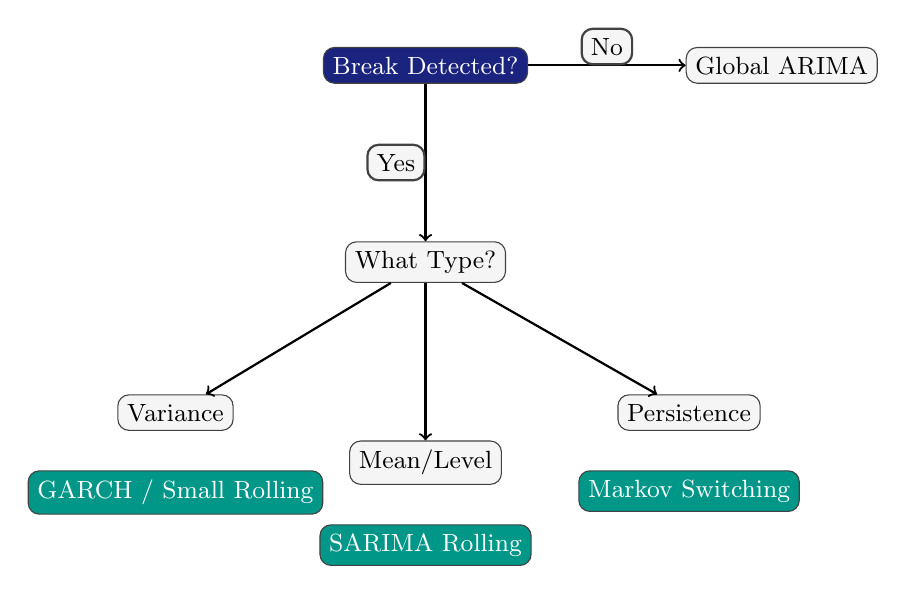
\begin{tikzpicture}[node distance=2cm, align=center, every node/.style={fill=SoftGrey, font=\small, draw=DarkGrey, rounded corners}]
      \node (start) [fill=MainBlue, text=white] {Break Detected?};
      \node (no) [right=of start] {Global ARIMA};
      \node (yes) [below=of start] {What Type?};
      
      \node (vol) [below left=of yes] {Variance};
      \node (mean) [below=of yes] {Mean/Level};
      \node (param) [below right=of yes] {Persistence};
      
      \node (garch) [below=0.5cm of vol, fill=AccentTeal, text=white] {GARCH / Small Rolling};
      \node (sarima) [below=0.5cm of mean, fill=AccentTeal, text=white] {SARIMA Rolling};
      \node (ms) [below=0.5cm of param, fill=AccentTeal, text=white] {Markov Switching};
      
      \draw[->, thick] (start) -- (no) node[midway, above] {No};
      \draw[->, thick] (start) -- (yes) node[midway, left] {Yes};
      \draw[->, thick] (yes) -- (vol);
      \draw[->, thick] (yes) -- (mean);
      \draw[->, thick] (yes) -- (param);
    \end{tikzpicture}
  \end{center}
\end{frame}

% 12. Conclusion
\begin{frame}{Key Contributions \& Summary}
  \begin{enumerate}
    \item \textbf{Comprehensive Framework:} Unified MC comparison of 15+ methods.
    \item \textbf{Seasonality Matters:} Bakhodir's SARIMA integration fills a real-world gap.
    \item \textbf{Adaptive Dominance:} Rolling windows and MS consistently beat global models.
    \item \textbf{Actionable Guidance:} Specific method recommendations based on break type.
  \end{enumerate}
\end{frame}

% 13. References
\begin{frame}[allowframebreaks]{Selected References}
  \nocite{stock1996, bai1998, bai2003, pesaran2013, rossi2013, hamilton1989, wang2013, antoshin2008}
  \bibliographystyle{apalike}
  \bibliography{bibliography}
\end{frame}

% 14. Thank You
\begin{frame}[plain]
  \begin{center}
    \vspace{2cm}
    \Huge \textcolor{MainBlue}{\textbf{Thank You!}} \\
    \vspace{1cm}
    \large \textbf{Questions?} \\
    \vspace{1.5cm}
    \footnotesize \texttt{github.com/qonlab/structural-break-forecasting}
  \end{center}
\end{frame}

\end{document}
